\documentclass[sigconf]{acmart}

\usepackage{booktabs} % For formal tables

\newif\iffinal

% Un-comment this line to see proposal without comments
%\finaltrue

\iffinal
  \newcommand\ian[1]{}
  \newcommand\kyle[1]{}
  \newcommand\bb[1]{}

\else
  \newcommand\ian[1]{{\color{blue}[Ian: #1]}}
  \newcommand\kyle[1]{{\color{red}[Kyle: #1]}}
  \newcommand\bb[1]{{\color{violet}[Blaiszik: #1]}}
\fi

% Copyright
%\setcopyright{none}
%\setcopyright{acmcopyright}
%\setcopyright{acmlicensed}
\setcopyright{rightsretained}
%\setcopyright{usgov}
%\setcopyright{usgovmixed}
%\setcopyright{cagov}
%\setcopyright{cagovmixed}

% DOI
\acmDOI{10.475/123_4}

% ISBN
\acmISBN{123-4567-24-567/08/06}

%Conference
\acmConference[PDSW-DISCS 2017]{2nd Joint International Workshop on Parallel Data Storage \& Data Intensive Scalable Computing Systems}{November 2017}{Denver, Colorado USA} 
\acmYear{2017}
\copyrightyear{2017}

\acmPrice{15.00}


\begin{document}
\title{Petrel: A Programmatically Accessible Research Data Service}

\author{William Allcock, Benjamin E. Allen, Rachana Ananthakrishnan,\\Ben Blaiszik, Kyle Chard, Ian Foster, Lukasz Lacinski, and Michael E. Papka}
\affiliation{%
  \institution{Argonne National Laboratory}
  \streetaddress{9700 S Cass Ave, Lemont, IL 60439, USA}
%  \city{Lemont} 
%  \state{IL} 
%  \postcode{60439}
}
\renewcommand{\shortauthors}{W. Allcock et al.}


\begin{abstract}
We report on our experiences deploying and operating Petrel,
a data service designed to support science projects 
that must organize and distribute large quantities of data.
Building on a high-performance 1.7~PB parallel file system and
embedded in Argonne National Laboratory's 100+ Gbps network fabric, Petrel 
leverages Science DMZ concepts and Globus APIs 
to provide application scientists with a high-speed,
highly connected, and programmatically controllable data store.
We describe Petrel's design, implementation, and usage and give
representative examples to illustrate the many different ways in which
scientists have employed the system. 
%
%Data-intensive science requires new data services beyond those provided by conventional
%high-performance computing (HPC) systems.
%We established the Petrel data server at Argonne National Laboratory in 2015 to experiment with the utility and operation of such services.
%This high-capacity, high-speed data store was configured to enable both interactive Web access
%and programmatic access via REST APIs and associated 
%
%Petrel is a data management service operated by the Argonne Leadership Computing Facility (ALCF)
%that allows researchers to store large datasets and easily share those data with collaborators. 
%%Researchers from the Argonne Leadership Computing Facility (ALCF) and Globus are developing the system collaboratively. 
%Petrel leverages ALCF
%storage and infrastructure and Globus transfer and sharing services to provide a mechanism for researchers to transfer data into the system, manage data on the filesystem, and share and transfer data to other locations. Authentication and identity to access the system is provided through Globus and users can access Petrel using their campus or institution federated login.
%We report here on the design, implementation, applications, and use of this service.
%\ian{The paper is to be submitted to \url{http://www.pdsw.org/index.shtml}. Five pages plus references. Due September 7, 11:59 PM, AOE. Need to fix index terms and keywords.}
\end{abstract}

%
% The code below should be generated by the tool at
% http://dl.acm.org/ccs.cfm
% Please copy and paste the code instead of the example below. 
%
%\begin{CCSXML}
%<ccs2012>
% <concept>
%  <concept_id>10010520.10010553.10010562</concept_id>
%  <concept_desc>Computer systems organization~Embedded systems\ian{TO FIX}</concept_desc>
%  <concept_significance>500</concept_significance>
% </concept>
% <concept>
%  <concept_id>10010520.10010575.10010755</concept_id>
%  <concept_desc>Computer systems organization~Redundancy</concept_desc>
%  <concept_significance>300</concept_significance>
% </concept>
% <concept>
%  <concept_id>10010520.10010553.10010554</concept_id>
%  <concept_desc>Computer systems organization~Robotics</concept_desc>
%  <concept_significance>100</concept_significance>
% </concept>
% <concept>
%  <concept_id>10003033.10003083.10003095</concept_id>
%  <concept_desc>Networks~Network reliability</concept_desc>
%  <concept_significance>100</concept_significance>
% </concept>
%</ccs2012>  
%\end{CCSXML}

%\ccsdesc[500]{Computer systems organization~Embedded systems}
%\ccsdesc[300]{Computer systems organization~Redundancy}
%\ccsdesc{Computer systems organization~Robotics}
%\ccsdesc[100]{Networks~Network reliability}


%\keywords{High-speed data service, }


\maketitle



\section{Introduction}

Data-intensive science increasingly requires discipline-based data management tools,
for example to distribute content from a curated repository, 
share files from a computational simulation or scientific instrument with collaborators,
enable analyses of hosted data by collaborators, 
or accept uploads for analysis or publication.
But would-be developers of such tools need a foundation on which to build:
a foundation that is not necessarily provided by 
conventional research computing facilities,
which are typically designed to support individual research projects 
rather than long-lived and community services.
They need, in particular,  
storage systems that provide substantial capacity and
high-speed storage and network access,
and that can be managed and accessed entirely programmatically
%(e.g., via REST APIs) 
for easy integration into domain-specific workflows.

These considerations led the Argonne Leadership Computing Facility (ALCF)
to establish the Petrel data service in 2015,
initially as an experiment to see whether and how people
might use a programmatically accessible storage service, 
and then---as success stories emerged---as a production
service for the scientific community.
The current Petrel system provides Globus %REST API  
access to 1.7~PB high-speed storage, 
connected to local and wide area networks
at 100+~Gbps.
%Users can authenticate by using their campus or institution federated login.
Users can request allocations of 100~TB or more.
If approved, they can then use Globus APIs (and associated Web interfaces) to  
move files to and from this allocated storage, organize files within this storage, and to authorize others to do the same. 
Petrel thus provides a configurable solution to the sharing of data with colleagues and the community, 
while at the  same time keeping large datasets close to large computational resources.

We have found the results of this experiment to be highly encouraging.
Dozens of groups have made use of Petrel in one way or another to transfer
data between Petrel and more than 600 remote locations.
Many groups have integrated its use into workflows, for example to
automate distribution of data from experimental facilities and to 
organize and share data from simulation campaigns.
%support computer science experiments ...
Petrel thus represents a way in which a high-performance computing facility such as ALCF can usefully evolve
beyond its traditional role of providing access to supercomputers for simulations~\cite{UrPa16}
to become a highly usable service facility. 
%deeply integrated into science projects and serving as a hub for science communities. 
Because Petrel is configured to integrate easily with user environments and workflows,
it can serve as a hub for science communities and 
improve the usability and utilization of the core HPC center. 

We report in subsequent sections on the design, application, and usage of the Petrel system
and reflect on lessons learned from its development and use.


%From a slide that I had on Petrel for ALCF review where we called it a data service
%
%ÒA uniform data fabric across the lab
%É with seamless access to large dataÉ
%É for use in computation, collaboration and distribution É
%É that is project focused and self 
%managed É
%É and is described and discoverableÓ


%modern research data portal   
%
%Providing such data acceleration services is a natural way for research computing centers to deliver enhanced value to their stakeholders. But implementing and operating such services can be expensive and cumbersome. 
%
%researchers often need to stage, store, share, and distribute large quantities of data.
%In response, we designed and deployed Petrel, 
%a data service designed to support scientific  
%
%programmatic access for automation 
%
%Conventional research computing facilities are rarely well suited for such purposes,
%being designed to support computational projects rather than data distribution.
%for example, a person may need an allocation and account before
%they can access a data system.
%
%Argonne National Laboratory is home to thousands of intramural scientists and also
%operates a variety of scientific user facilities,
%including both experimental apparatus such as the Advanced Photon Source,
%with its more than 60 beamlines, and supercomputers, such as those operated
%by the Argonne Leadership Computing Facility.
%These facilities are used by many thousands of scientists annually, who increasingly
%face the need 
%These facilities and other activities at the lab increasingly involve large 
%quantities of data, 
%which proved to be surprisingly difficult to manipulate due to the lack of suitable storate facilities 
%




%\begin{verbatim}
%32 Nodes with 1.7 PB usable storage
%GPFS and Globus
%100TB allocation per project
%Transfer and sharing data with collaborators
%Federated login
%Self-managed by PIs
%\end{verbatim}




%Transfers to/from Petrel 80027
%Transfers from Petrel 59018
%Transfers to Petrel 21304
%Transfers within Petrel 295
%Unique src EPs 281
%Unique dst EPs 522
%Unique EPs 649
%Total data from Petrel 2.07274415613e+15
%Total files from Petrel 72779854.0
%Total data to Petrel 4.13027153675e+15
%Total files to Petrel 255731042.0
%Total data to/from Petrel 6.1187793935e+15
%Total files to/from Petrel 326728415.0



\section{The Petrel System}

Historically,
data at high-performance computing (HPC) centers have been located either on parallel file systems
designed for rapid \emph{internal} access or on data portal servers that support slower \emph{external} data distribution;
only the latter traffic was allowed to traverse the firewall.
Thus 
high-speed data movement in and out of HPC centers was often difficult.
Furthermore, collaboration in such environments has in the past been equally difficult, as 
users had to request or create accounts for each of their collaborators---a process
that was often cumbersome and not flexible enough to support dynamic collaborations. 
 
A recent reinvention of academic network architectures introduces the 
concept of a Science DMZ~\cite{dart2014science}, 
in which specialized data servers are connected directly to
high-speed networks and storage systems.  
This development has allowed for the emergence of the \textbf{modern research data portal} (MRDP) design pattern~\cite{BMRDP},
in which 
%portal functionality is decomposed along two distinct but complementary dimensions.
%First, 
control channel communications and data channel communications are separated,
with the former handled by a web server computer deployed (most often) in the institution's enterprise network
and the latter by specialized data servers connected directly to high-speed networks
and storage systems.
The MRDP design pattern also simplifies implementation of data portal functionality by outsourcing
%Second, 
responsibility for managing data transfers, data access, and sometimes also authentication
to external, often cloud-hosted, services, such as Globus.
Thus data portal implementations can use simple REST API calls to manage data access.
%The design pattern thus defines distinct roles for the web server, 
%which manages who is allowed to do what;
%data servers, where authorized operations are performed on data;
%and external services, which orchestrate data access. 

Petrel is designed to support the deployment
and operation of instances of this MRDP design pattern and other similar applications that need to
manage data movement through
a highly connected, high-speed data store.
It provides a user-oriented, collaborative storage model in which
users manage their own isolated storage allocations including not
only data organization but also dynamic sharing of files and directories
within the allocation without requiring local user accounts.
A central characteristic is its support for API access, which allows
sophisticated behaviors to be implemented with modest amounts of programming.
In the following, we first describe the Petrel hardware and then the use of Globus services   
for managing access, data transfers, and data sharing.


\begin{figure}
\centering
%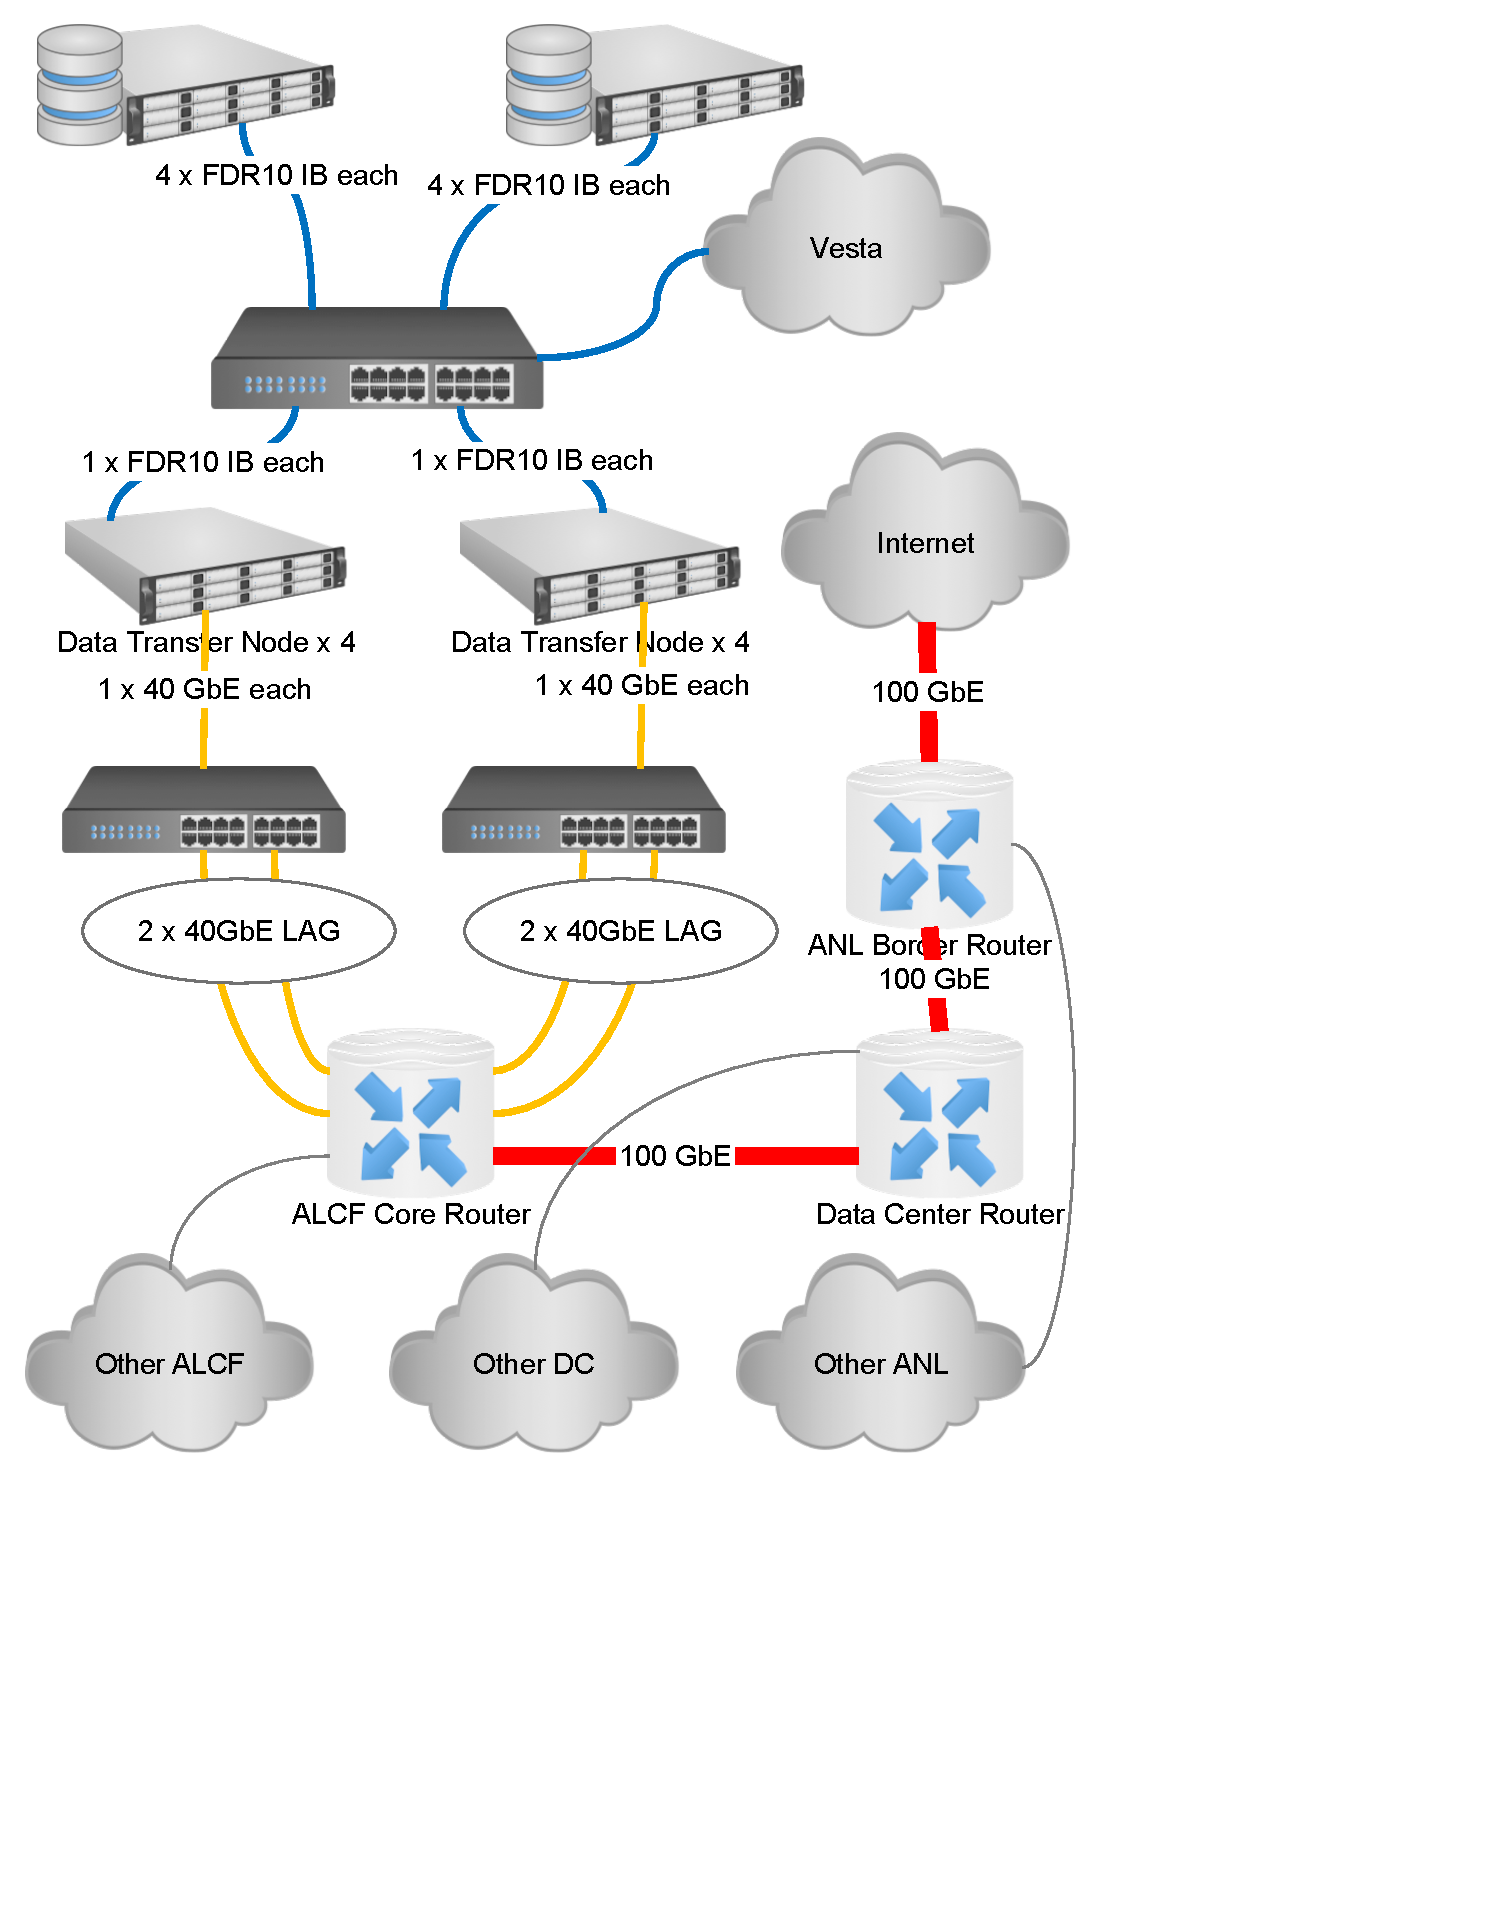
\includegraphics[trim=0.1in 3in 2.7in 0,clip,width=\columnwidth]{Figures/PetrelSystemDiagramNarrow.pdf}
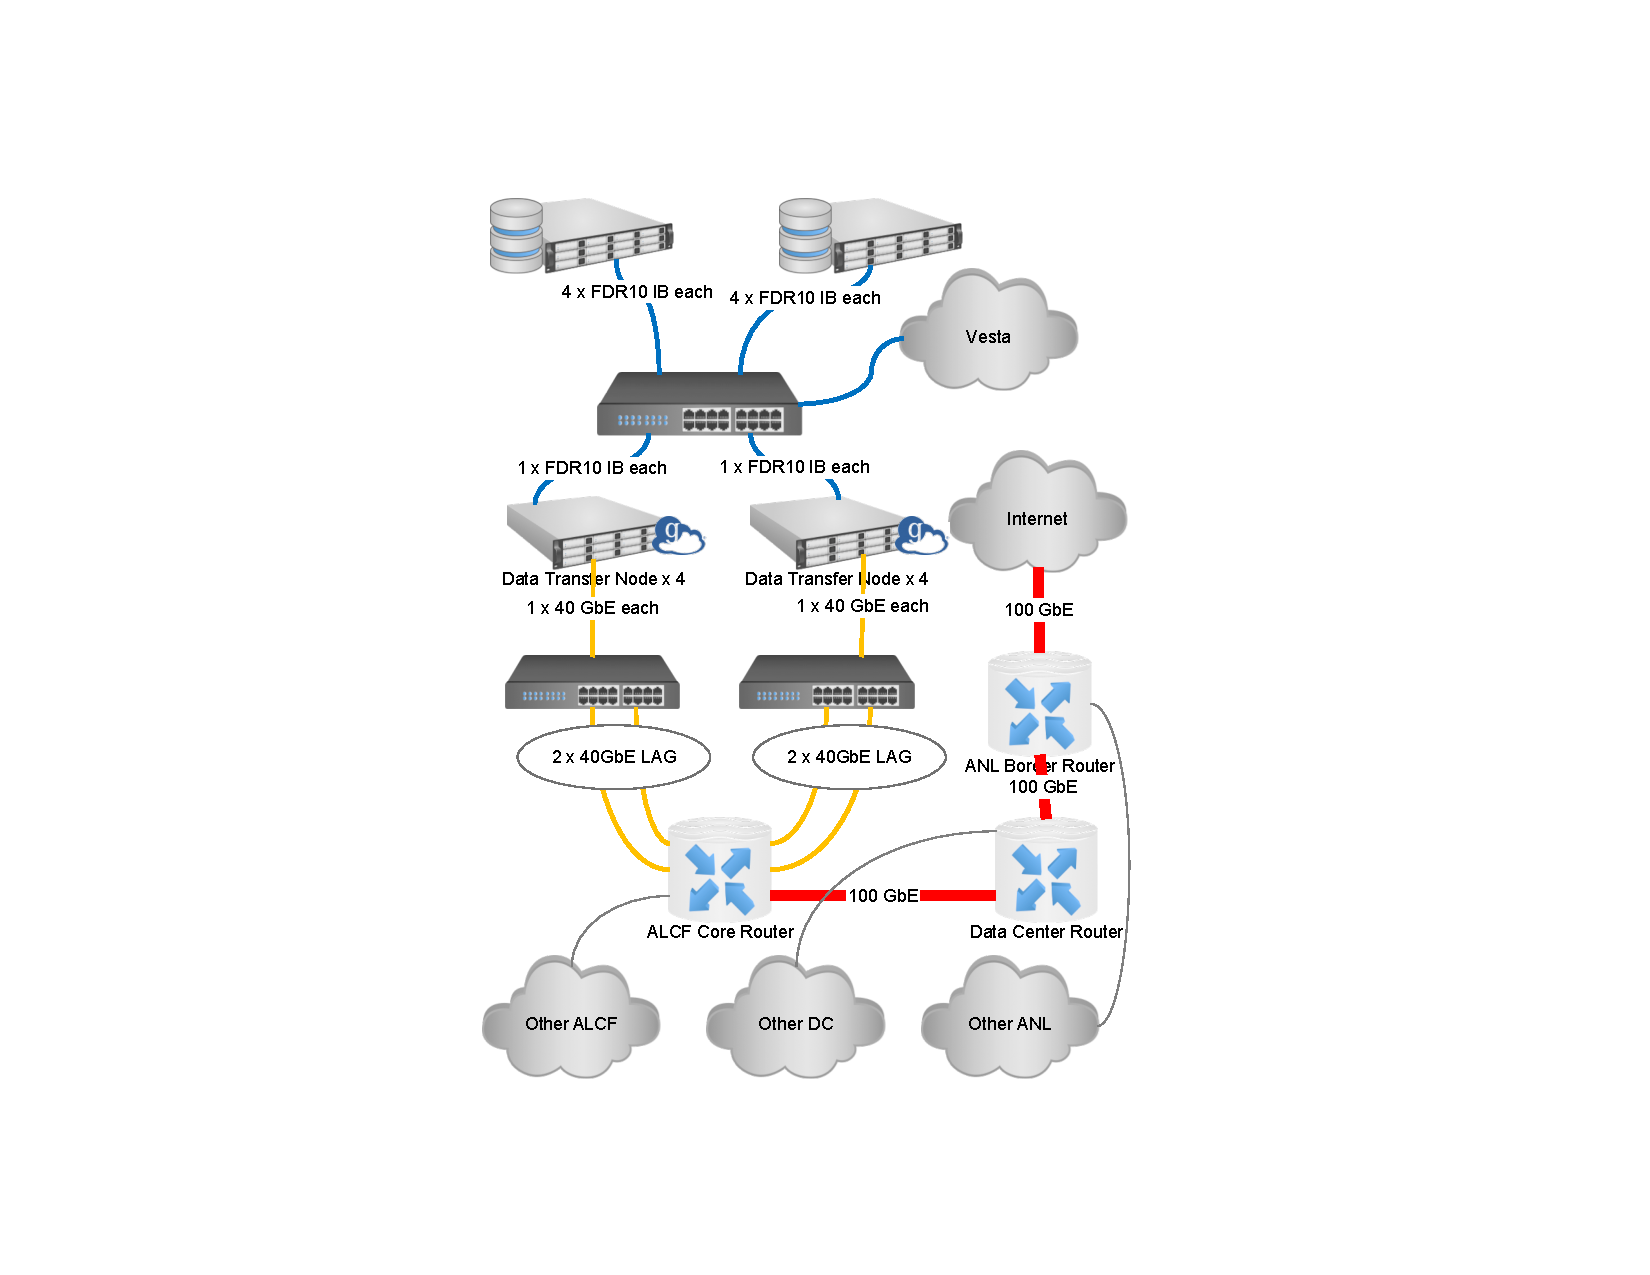
\includegraphics[trim=3.2in 1.3in 3.4in 1.3in,clip,width=\columnwidth]{Figures/PetrelSystemDiagramNarrowG.pdf}

\vspace{-1ex}

\caption{Petrel architecture, as described in the text. The NSD servers are at the top,
with the DTNs are below them. The remainder of the figure shows how Petrel is connected to
ALCF, other data center, and remote networks. \label{fig:arch}}
\end{figure}


\subsection{The Petrel Data Store and DTNs}

The Petrel system comprises a parallel file system running the
IBM Spectrum Scale file system (formerly known as the
General Parallel File System, GPFS~\cite{schmuck2002gpfs}),
plus eight associated data transfer nodes (DTNs)~\cite{dart2014science} for remote access. 
This hardware is configured to operate as a Science DMZ, 
meaning that it is accessible from external networks without passing through the usual firewalls.
Line-rate firewalls are in place,
configured 
with network access control lists 
to limit access to Globus/GridFTP ports and,
in particular, to limit control channel access to Globus service IP addresses.

%Petrel hardware comprises a single IBM Elastic Storage Server (ESS) GL6 plus eight DTNs for external access.

The Petrel data store currently comprises  a single IBM Elastic Storage Server (ESS) GL6.
This device is configured with two IBM S822L Power8 based servers as IBM Spectrum Scale Network Shared Disk (NSD) servers, and one IBM S812L as a management and provisioning server. 
Each NSD server is connected with 4$\times$FDR10 connections to the same fabric as the DTNs. 
Petrel includes six disk trays with a total of 348 6TB SAS HDDs. 
Configured with 8+2 parity and 3 drives worth of hot spare space, 
Petrel provides a usable capacity of 1.7P, and has been benchmarked via IOR at a maximum write rate of 16,563 MiB/sec (17,368 MB/sec) and maximum read rate of  23,111 MiB/sec (24,233 MB/sec).

Each of the eight Petrel DTNs has a single Mellanox ConnectX-4 40GbE NIC, a single Mellanox Connect-IB HBA (running at QDR), 64GB RAM ($\sim$42GB dedicated to Spectrum Scale), and a single socket Intel E5-1660 v3 8c @ 3.00GHz CPU. 
Both Mellanox cards sit on PCIe 3.0 x16 buses.

The eight Petrel DTNs are connected to two core Mellanox SX1710 36-port 40GbE switches
maintained within Argonne's Joint Laboratory for Systems Evaluation (JLSE).
%JLSE has two core Mellanox SX1710 36-port 40GbE switches. 
The Petrel DTNs are split across the two switches, each connected with 1$\times$40GbE. 
%The split is along even and odd numbered DTNs. 
Each of the two 40GbE core switches has a 2$\times$40GbE link aggregation group to the ALCF core router, which in turn has a 100GbE connection to the core router for the data center within
which ALCF is located,
%SDN240. 
%At this point we are sharing available bandwidth with ALCF. 
%SDN240 in turns 
which in turn connects at 100GbE to one of the ANL border routers.
Thus, as Petrel traffic reaches beyond JSLE to ALCF, the data center, and the border,
it shares bandwidth with an increasing range of other activities.
%At this point we share available bandwidth with all of the 240 datacenter, 
%and at the border we share with the rest of the lab to ESNet.

\subsection{Globus Remote Access Services}

Remote access to Petrel capabilities
is provided via Globus services~\cite{Globus2016}.
Globus provides data and identity management capabilities designed for the research community. 
These capabilities are delivered via a cloud-hosted software- and platform-as-a-service model, 
enabling users to access them through their web browser and
developers to invoke them via powerful APIs. 
We describe here Globus capabilities for managing and transferring data and for authenticating users and authorizing access.

Globus allows data to be remotely managed across its pool of more than 10,000 accessible storage systems (called ``endpoints''). 
A storage system is made accessible to Globus, and thus capable of high performance and reliable data transfer, by installing Globus Connect software. 
Globus Connect is offered in two versions: 
Globus Connect Personal for single-user deployments (e.g., a laptop or PC) and Globus Connect Server for multi-user
deployments (e.g., a shared server or DTN). 
Globus Connect can be deployed across multiple physical servers to enable
parallel (``striped'') data transfers and enhance reliability by allowing for dynamic failover. 
Petrel runs Globus Connect Server software on its eight DTNs.

Globus Transfer capabilities provide high performance and reliable third party data transfer. 
The Globus service manages the entire transfer process, including coordinating authentication at source and destination; establishing a high performance data channel using  the GridFTP protocol, with configuration optimized for transfer; ensuring data integrity by comparing source/destination checksums; and recovering from any errors during the transfer.  Globus, by default, enforces the data access permissions represented
by the underlying system; however, it also allows these access decisions to be managed through the cloud service. In the latter mode, called Globus Sharing, users may associate user- or group-based access control lists (ACLs) with particular file paths. Globus checks and enforces these ACLs when other users attempt to read or write to those paths.

Globus Sharing is at the heart of Petrel. Each petrel allocation is assigned
a unique shared endpoint. The owner of the allocation is given admin privileges
on that shared endpoint which enable them to not only to manage data on
that endpoint but to also select which other users may access or manage the endpoint. 
Globus Sharing operates entirely with Globus Auth identities, that is it does
not require that administrators or users of a shared endpoint have local accounts. 
Further, it implements advanced security models to, for example, pair
a shared endpoint with its root directory, restrict what paths can 
be shared, and to hide any details of paths beyond what is shared in the
file system hierarchy.

Globus Auth~\cite{tuecke16auth} provides identity and access management platform capabilities. It brokers authentication and authorization interactions between end-users, identity providers, resource servers (services), and clients (e.g., web, mobile, desktop, and command line applications, and other services). 
It implements standard web protocols, such as OAuth 2.0 and OpenID Connect, that allow it to be integrated easily with external applications using standard client libraries. 
These protocols enable third-party applications to authenticate users (using their preferred identity) directly with the chosen identity provider. Globus Auth then returns access
tokens that the third-party application can use to validate the user's identity and to perform actions on behalf of that user, within an agreed upon scope. Globus Auth implements an identity federation model via which diverse identities can be linked, and such that presentation of one identity may support authorization for the set of identities. 

Globus Groups~\cite{chard16nexus} provides a user-managed hierarchical group management service. 
It is most often used to implement group-based authorization and to allow
users to manage collections of other users. Petrel relies on Globus
Groups to define the set of users who are able to manage and access
a particular allocation.

\section{Example User Workflows}

Any scientist with an Argonne affiliation can request a project allocation on Petrel. 
Upon approval, they have access to 100TB which they can access via Globus
web interface and REST APIs, either directly or by using associated Python software development kits (SDKs).
They can transfer data to and from Petrel, create and delete directories and shared endpoints,
and grant other users rights to manage, read, and/or write the space.

We provide quantitative data on usage in Section~\ref{sec:usage}.
Here we review a few representation examples of specific applications that make use or,
or that were developed specifically for, Petrel. 


%Once data are generated at APS, scientists transfer them to the project space on Petrel. 
%They can then set up permissions to enable remote collaborators to access all or a subset of the data. 
%Importantly, remote collaborators do not need Argonne accounts to access the data.
%
%Petrel users can easily stage all or some of their data to a compute resource for analysis, and then move results back to Petrel.
%

\subsection{Light Source Data Distribution}

The Advanced Photon Source (APS) at Argonne National Laboratory, like many experimental facilities
worldwide, 
serves thousands of researchers every year, 
%most of whom collect data and return to their home institution.
most of whom visit just for a few days to collect data and then return to their home institution.
In the past, data produced during an experiment were invariably carried back on physical media.
However, as data sizes have grown and experiments have become more collaborative,
that approach has become less effective.
Data transfer via network is preferred;
the challenge is to integrate data transfer into the experimental workflow of the facility
in a way that is automated, secure, reliable, and scalable. %to thousands of users and datasets.

%Francesco De Carlo has used Globus APIs to do just that.
The DMagic system (\url{dmagic.readthedocs.io}) used Petrel to do just that. %implements a variant of the program in Listing~\ref{fig:rdpcode}
%It integrates with APS administrative and facility systems to deliver data to experimental users.
%When an experiment is approved at the APS, the associated researchers are registered in an APS database.
%a set of associated researchers are registered in the APS administrative database as approved participants.
%DMagic leverages this information as follows.
DMagic integrates with APS administrative and facility systems to deliver data to experimental users.
Before the experiment begins,
it uses a Globus API to create a shared endpoint on Petrel,
%a large storage system maintained by Argonne's computing facility.
retrieves from the APS scheduling system 
the list of approved users for the experiment, and uses further Globus API calls to
add permissions for those users to the shared endpoint.
It subsequently monitors the experiment data directory at the APS experimental facility and copies
new files automatically to that shared endpoint,
from which they can be retrieved by any approved user.

DMagic is now used by several APS beamlines to
track study metadata and provenance, 
and to share raw and analyzed data with local and remote collaborators.
For example, a
microtomography beamline currently collects 20--80 TB/month of raw data and expects to scale to about 100--200 TB/month in the near future. 
Petrel is being used in workflows that involve streaming analysis of data as it is collected~\cite{bicer2016optimization} with the TomoPy toolkit~\cite{gursoy2014tomopy},
and for experiments in rule-based data collection and processing~\cite{chard2017ripple}. 
%Microtomography can be carried out at a variety of energies suitable for 3D characterization of materials relevant to materials science, geoscience, energy storage, and biology. 
%High-speed imaging allows for ultra-short exposure times, allowing for detailed study of transient material phenomena. 
%Researchers in this group get an allocation at the beamline for a duration of a few days, and gather data that needs to be further processed and analyzed. 
%Subsets of the raw data need to be moved to a diverse set of analysis and storage facilities for processing and long-term preservation. 
%Users can leverage Petrel to help meet these requirements. 



\subsection{Materials Science}

Scientists from Argonne's Materials Science Division gather experimental data from APS beamlines.
Raw data volumes range from 60--100 TB/month. 
%They require a flexible environment to implement end-to-end experiment-time data analysis workflows to automate their analyses and leverage distributed computing resources. This functionality allows the researchers to compare their experimental data to simulation results drawn from high-performance computing resources to rapidly provide actionable feedback and data visualization. These scientists leverage Petrel to help meet these requirements.
They use Petrel and Globus functionality to share, bundle, and publish datasets~\cite{foster2015networking}. 
They also integrate Petrel into workflows that make datasets accessible for remote visualization
from Python clients~\cite{wozniak2015big}. 

After data are gathered, the scientists often want to share subsets of raw data, derived datasets, and analysis results with collaborators, track metadata associated with the data, and track data provenance. 
Eventually, these scientists may want to make their datasets publicly and persistently available via publication functionality~\cite{chard2015globus}, 
fully bundled with the associated metadata and associated with a persistent identifier to aide search, discovery, and data citability.

\subsection{Materials Data Facility}

The Materials Data Facility (MDF)~\cite{MDF2016} provides the materials science community
with data services for simplified publication, discovery, and reuse of materials-related datasets. 
Its data publication service allows researchers to 
publish datasets stored on distributed resources (i.e., any Globus endpoint), mint permanent unique identifiers 
(e.g., DOI or Handle), and operate data publication workflows through a web interface or API~\cite{chard2015globus}. The MDF data discovery service provides 
a simple query API along with Python tools to help users find and access full datasets published in MDF as well as  discover links to a host of relevant data indexed 
from a variety of external efforts (117 sources indexed to date). 

MDF leverages the Petrel service to: 
1) share collaborative spaces with research teams across the country for use in collecting and organizing project 
data prior to final publication and sharing with the public;
2) stage datasets for indexing into the MDF discovery service (currently $\sim$60 TB of data); and
3) store a raw copy of the extracted JSON-formatted metadata for index persistence. 

In the future, the
MDF team is interested in attaching compute resources to Petrel in order to streamline operations on  
the stored datasets. 
These operations may include indexing material-specific file contents, extracting general metadata, performing analyzing and modeling tasks, visualizing dataset components, submitting jobs to other
ALCF resources, or interacting with the data via applications such as Jupyter~\cite{kluyver2016jupyter}.

\subsection{Other applications}

Petrel file system data and metadata have been used in studies of rule-based data management~\cite{chard2017ripple} and 
automated type inference and metadata extraction~\cite{beckman2017skluma},
and for data transfer modeling and optimization studies~\cite{liu2017explaining}. 
In each case, the ability to write programs that stage data on high-speed storage 
has proved useful.

The DOE's Energy Exascale Earth System Model project (formerly ACME)~\cite{schmidt2017practice}
uses Petrel to share large climate simulation data, including those published via the Earth System Grid~\cite{doi:10.1175/2008BAMS2459.1}.

%\kyle{It might not be so interesting, but we also use it for Globus labs.}

\section{Usage Data}\label{sec:usage}

Petrel has operated in its current configuration since July 14, 2014.
(A first version, constructed with repurposed hardware from the Intrepid supercomputer, 
used 32 1~Gbps-connected DTNs and DDN S2A9900 storage systems.)
During that time, it has been used to perform 
80,349 transfers (59,165 outbound, 21,479 inbound),
comprising 6.19~PB (2.10~PB outbound, 4.18~PB inbound) and 328M files (73M outbound, 256M inbound).
(Numbers do not add up perfectly due to a few hundred transfers from Petrel to Petrel.)
Usage is distributed across the Globus web interface (12,203 transfers), Globus Command
Line Interface (22,487 transfers), and REST APIs (45,659 transfers).
A total of 663 unique endpoints have communicated with Petrel, 285 as sources and 534 as destinations. 
Figure~\ref{fig:usage1} shows that these endpoints are located primarily in the US and Europe, but also
encompass Asia and Australia. 
%(Many endpoints located within Argonne National Laboratory are not visible on the map as their distance
%from Petrel is too small.)

Figure~\ref{fig:usage2} provides some perspectives on Petrel usage and performance.
Each point in this graph represents a single transfer, often encompassing multiple files but
managed as a unit.
The x-axis represents the great circle distance between Petrel and the remote source or destination
and the y-axis, with a log scale, the number of bytes involved in the transfer.
From left to right, we see many transfers within the US, a considerable number to Europe
(the great circle distance from Chicago to London is 6,300 km),
and significant numbers even to yet more distant locations.
Looking at sizes, we see many transfers of more than a terabyte and one close to a petabyte, 
but the majority quite a bit smaller.
Transfer rates also vary considerably.
They are in general lower for smaller and more distant transfers;
the highest observed was 40 Gbps (5 GB/s) disk-to-disk %(and 73 Gbps memory-to-memory)
from the University of Chicago's Research
Computing Center.     
Given that Petrel is itself optimized for high-speed transfers,
we can expect that, as observed in other studies~\cite{allcock2005globus,ito2005parameter,kim2015highly,yildirim2016application,liu2017explaining}, 
the rate for any particular transfer will depend largely 
on the characteristics of the transfer and the remote endpoint, and on
the volume of contending transfers.  

Figure~\ref{fig:ratesize} shows data size vs transfer rate for 
transfers that originate or end at Petrel. The graph shows
particular emphasis on large-scale and high performance data
transfers coming into and out of Petrel. Outgoing transfers
are in general more variable with respect to size and transfer
rate as there are significantly more outgoing transfers and 
significantly more destination endpoints. 
Figure~\ref{fig:perday} highlights the consistent use of Petrel
on a daily basis over the past three years. This figure
shows, on average, transfers of between 10 GB and 1 TB per day.



%Here are the stats you asked for:
% 
%Transfers to/from Petrel: 80027
%Transfers from Petrel: 59018
%Transfers to Petrel: 21304
%Transfers within Petrel: 295
% 
%Unique from Eps: 281
%Unique to Eps: 522
%Unique Eps: 649
% 
%Eps mapped to location: 639 (/649)
% 
%Transfers
%No to location: 259
%No from location: 885
% 
%Zero km to Petrel: 16133
%Zero km from petrel: 6375
% 
%Total transfers after removing Eps where we donÕt have a location and transfers with 0 km distance
%Total to Petrel: 4912 (/21304)
%Total from Petrel: 51758 (/59018)

Petrel has proved to be highly reliable: only one hard drive has failed 
since it was put into production, in July 2017.
(One other drive failed during early burn-in.)

%Here is a list of all Petrel projects (excepting test or demo projects),
%disk space usage, with an organization and department of a PI of each
%project:

%37T     2idb (Argonne National Laboratory; Advanced Photon Source/X-ray
%Science Division)
%4.3T    ACME (Argonne National Lanboratory; MCS)
%12T     alpha-nek (University of Chicago; Physics)
%3.6T    CODAR (Argonne National Lanboratory; MCS)
%89T     Discovery Engines for Big Data  (Argonne National Laboratory; MCS)
%674M    Discovery Engines LDRD (Argonne National Laboratory;
%MCS/Computation Institute)
%0       ECP-Candle (University of Chicago; CELS)
%13T     EWN (University of Chicago; Computation Institute)
%42T     Fuel Spray (Argonne National Laboratory; XSD/TRR)
%5.6T    gixs (Argonne National Laboratory; Advanced Photon Source)
%195G    Globus (Argonne National Laboratory; MCS)
%0       Globus bandwidth testing (National Institutes of Health; NIH HPC)
%2.4T    globuslabs (University of Chicago; Computation Institute)
%142T    globusperformancetesting (University of Chicago; Globus)
%39G     globuspublish (University of Chicago; Computation Institute)
%0       IMCA data transfer (AbbVie Inc; AbbVie IR)
%51T     NRCM_DD (Argonne National Laboratory; EVS)
%0       Patric (Argonne National Laboratory; CELS)
%59T     Research Data Analytics (Argonne National Laboratory/University
%of Chicago; CELS-Computation Institute)
%53G     RSPrec  (NRL; Plasma Physics)
%38G     SBC-CAT Data Management (Argonne National Laboratory; Advanced
%Photon Source)
%37G     SDM (Argonne National Laboratory; Advanced Photon Source)
%30G     Small Worlds (Argonne National Laboratory; Argonne Leadership
%Computing)
%1.1T    Structural Biology Data Grid (Harvard Medical School; BCMP)
%481T    tomography (Argonne National Laboratory; Advanced Photon Source)
%84T     xbrainmap (Argonne National Laboratory; Advanced Photon Source)
%26T     xfm (Argonne National Laboratory; Advanced Photon Source)
%154T    XPCS (Argonne National Laboratory; Advanced Photon Source)
%0       X-ray ptychography (Argonne/Northwestern; APS)
%
%25 projects (out of all 29) stored data
%Total file system usage: 1.3 PB



\begin{figure}
\centering
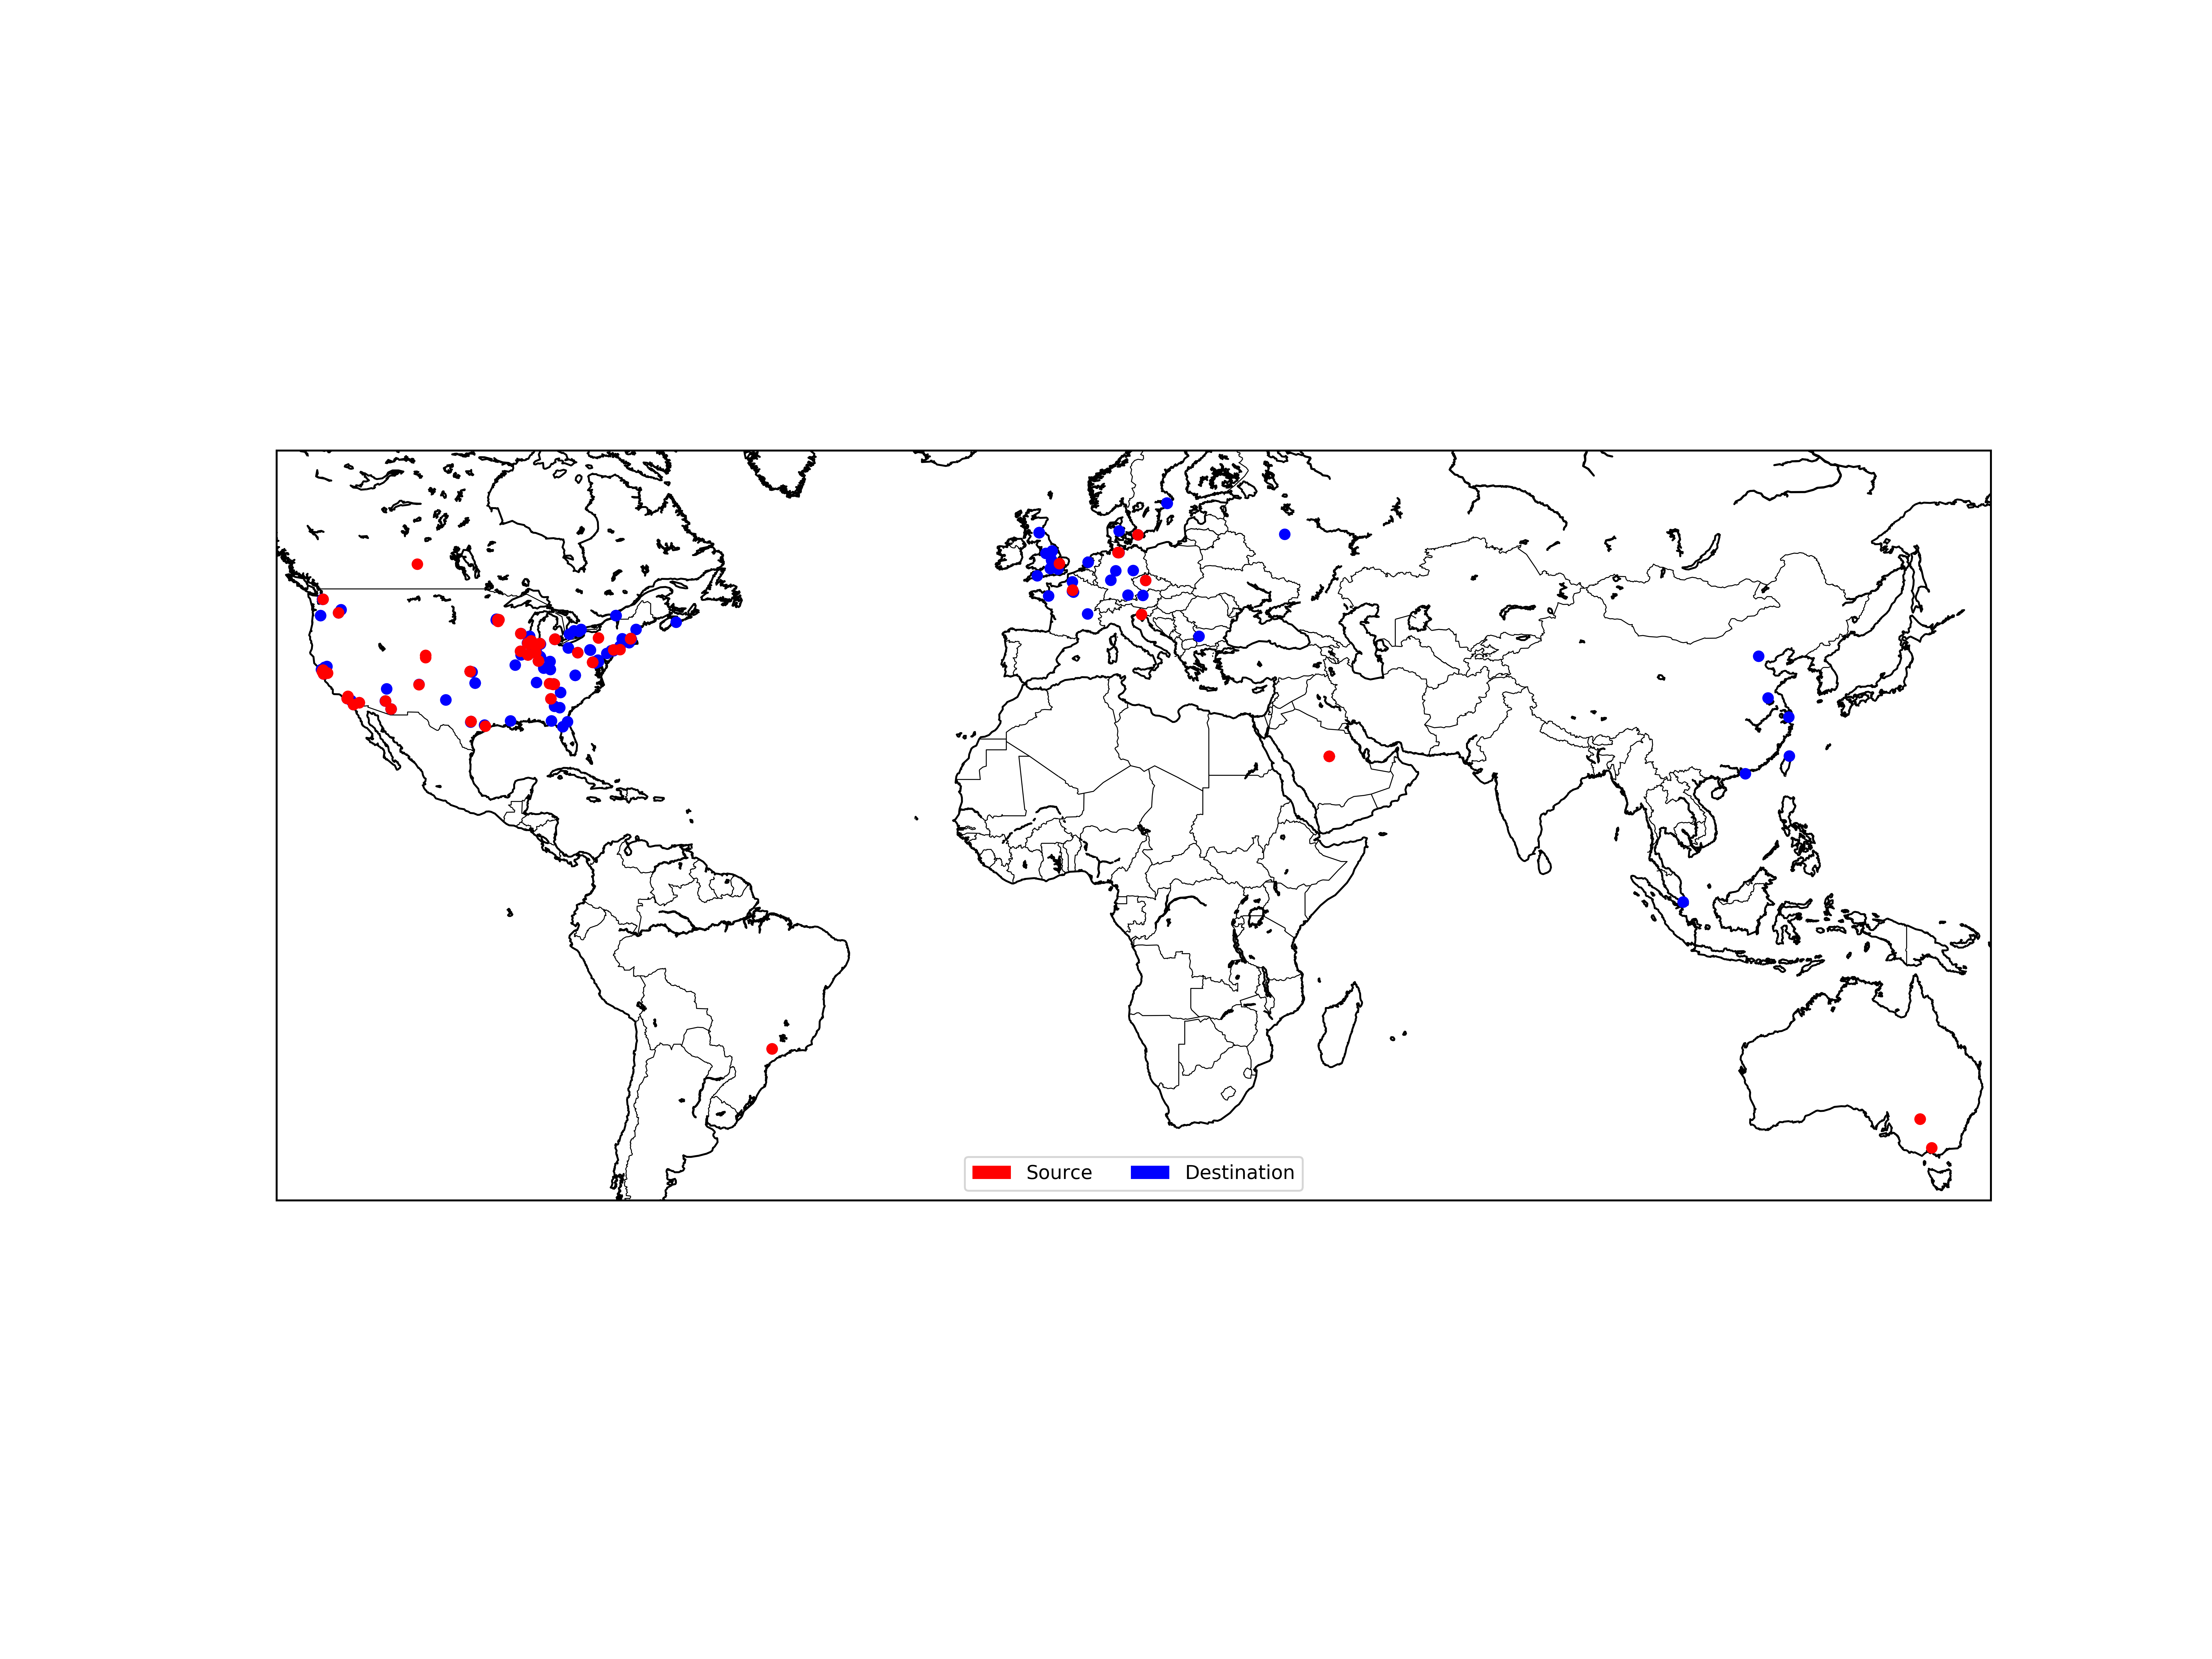
\includegraphics[trim=2in 3.3in 1.4in 3in,clip,width=\columnwidth]{Figures/petrel-src-dst-map-3.png}

\vspace{-1ex}

\caption{The 640 (of 663 total) Petrel source and destination endpoints for which geolocation
data are available.\label{fig:usage1}}
\end{figure}


\begin{figure}
\centering
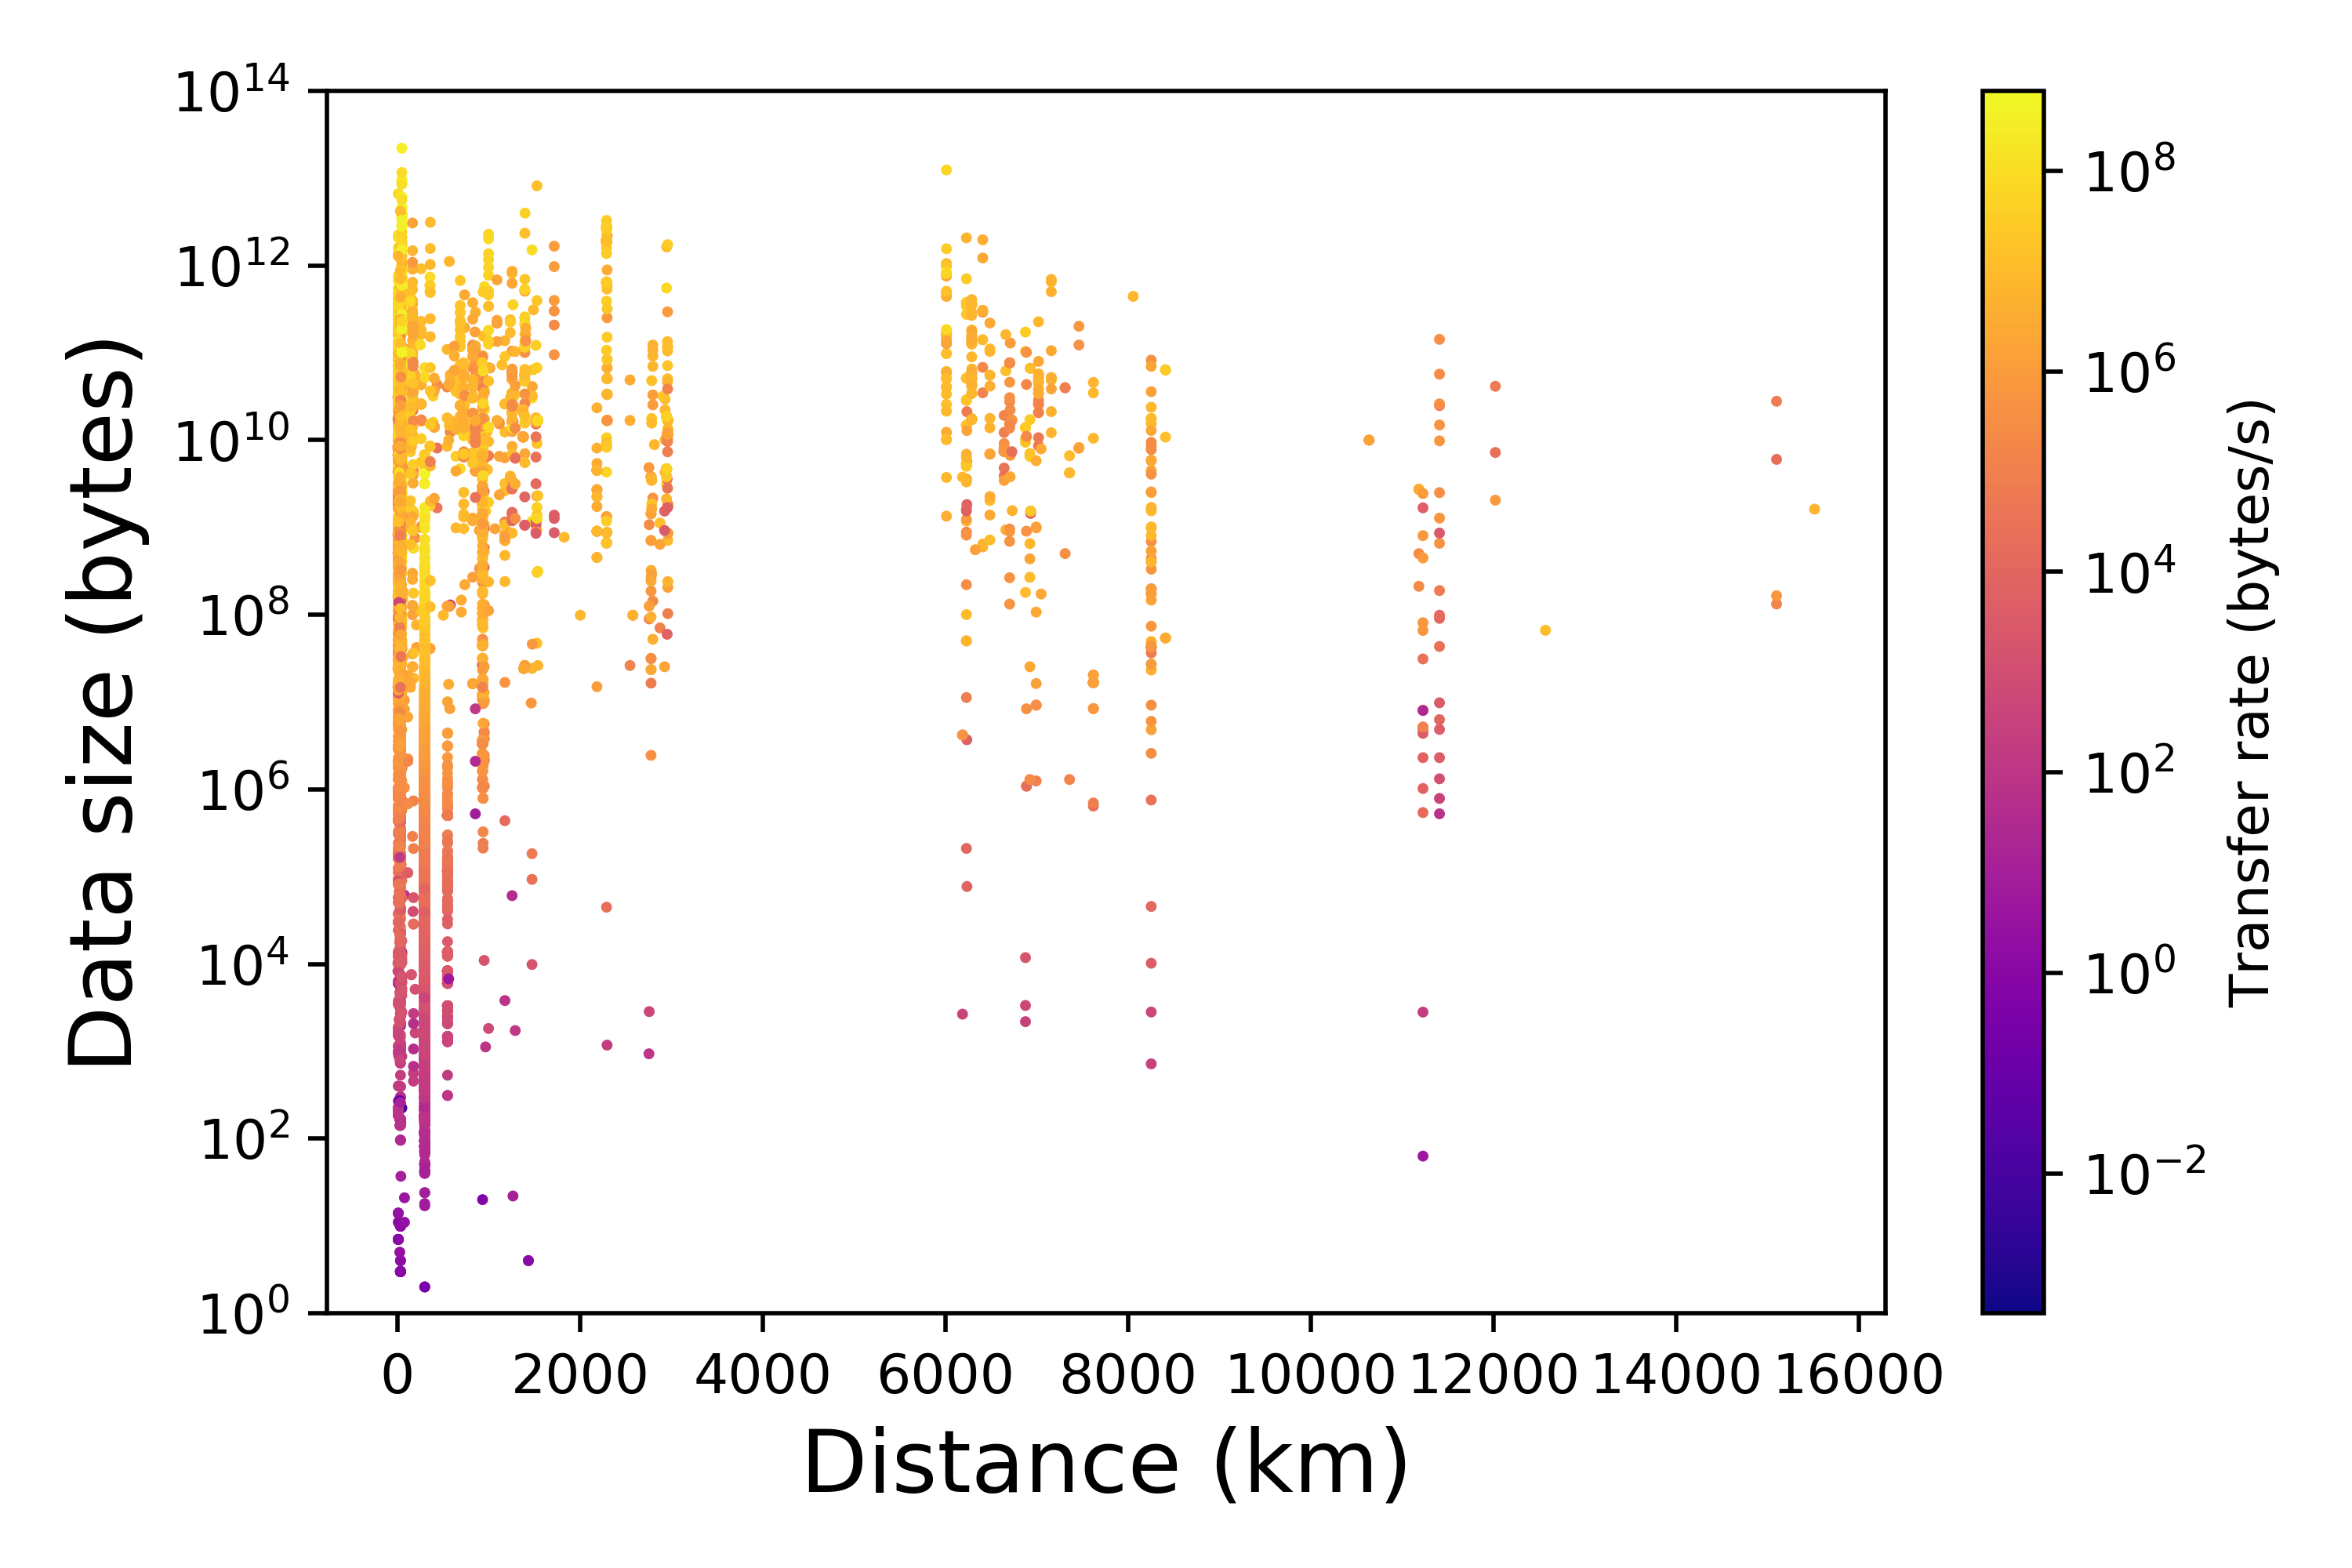
\includegraphics[trim=0.19in 0.1in 0.2in 0.1in,clip,width=\columnwidth]{Figures/size-distance-speed.png}

\vspace{-2ex}

\caption{The 79,415 transfers with Petrel as source or destination
for which geolocation data are available. Each point represents a single transfer,
and gives size vs.\ great circle distance between Petrel and remote source or destination, 
with transfer rate color coded.\label{fig:usage2}}
\end{figure}

\begin{figure}
\centering
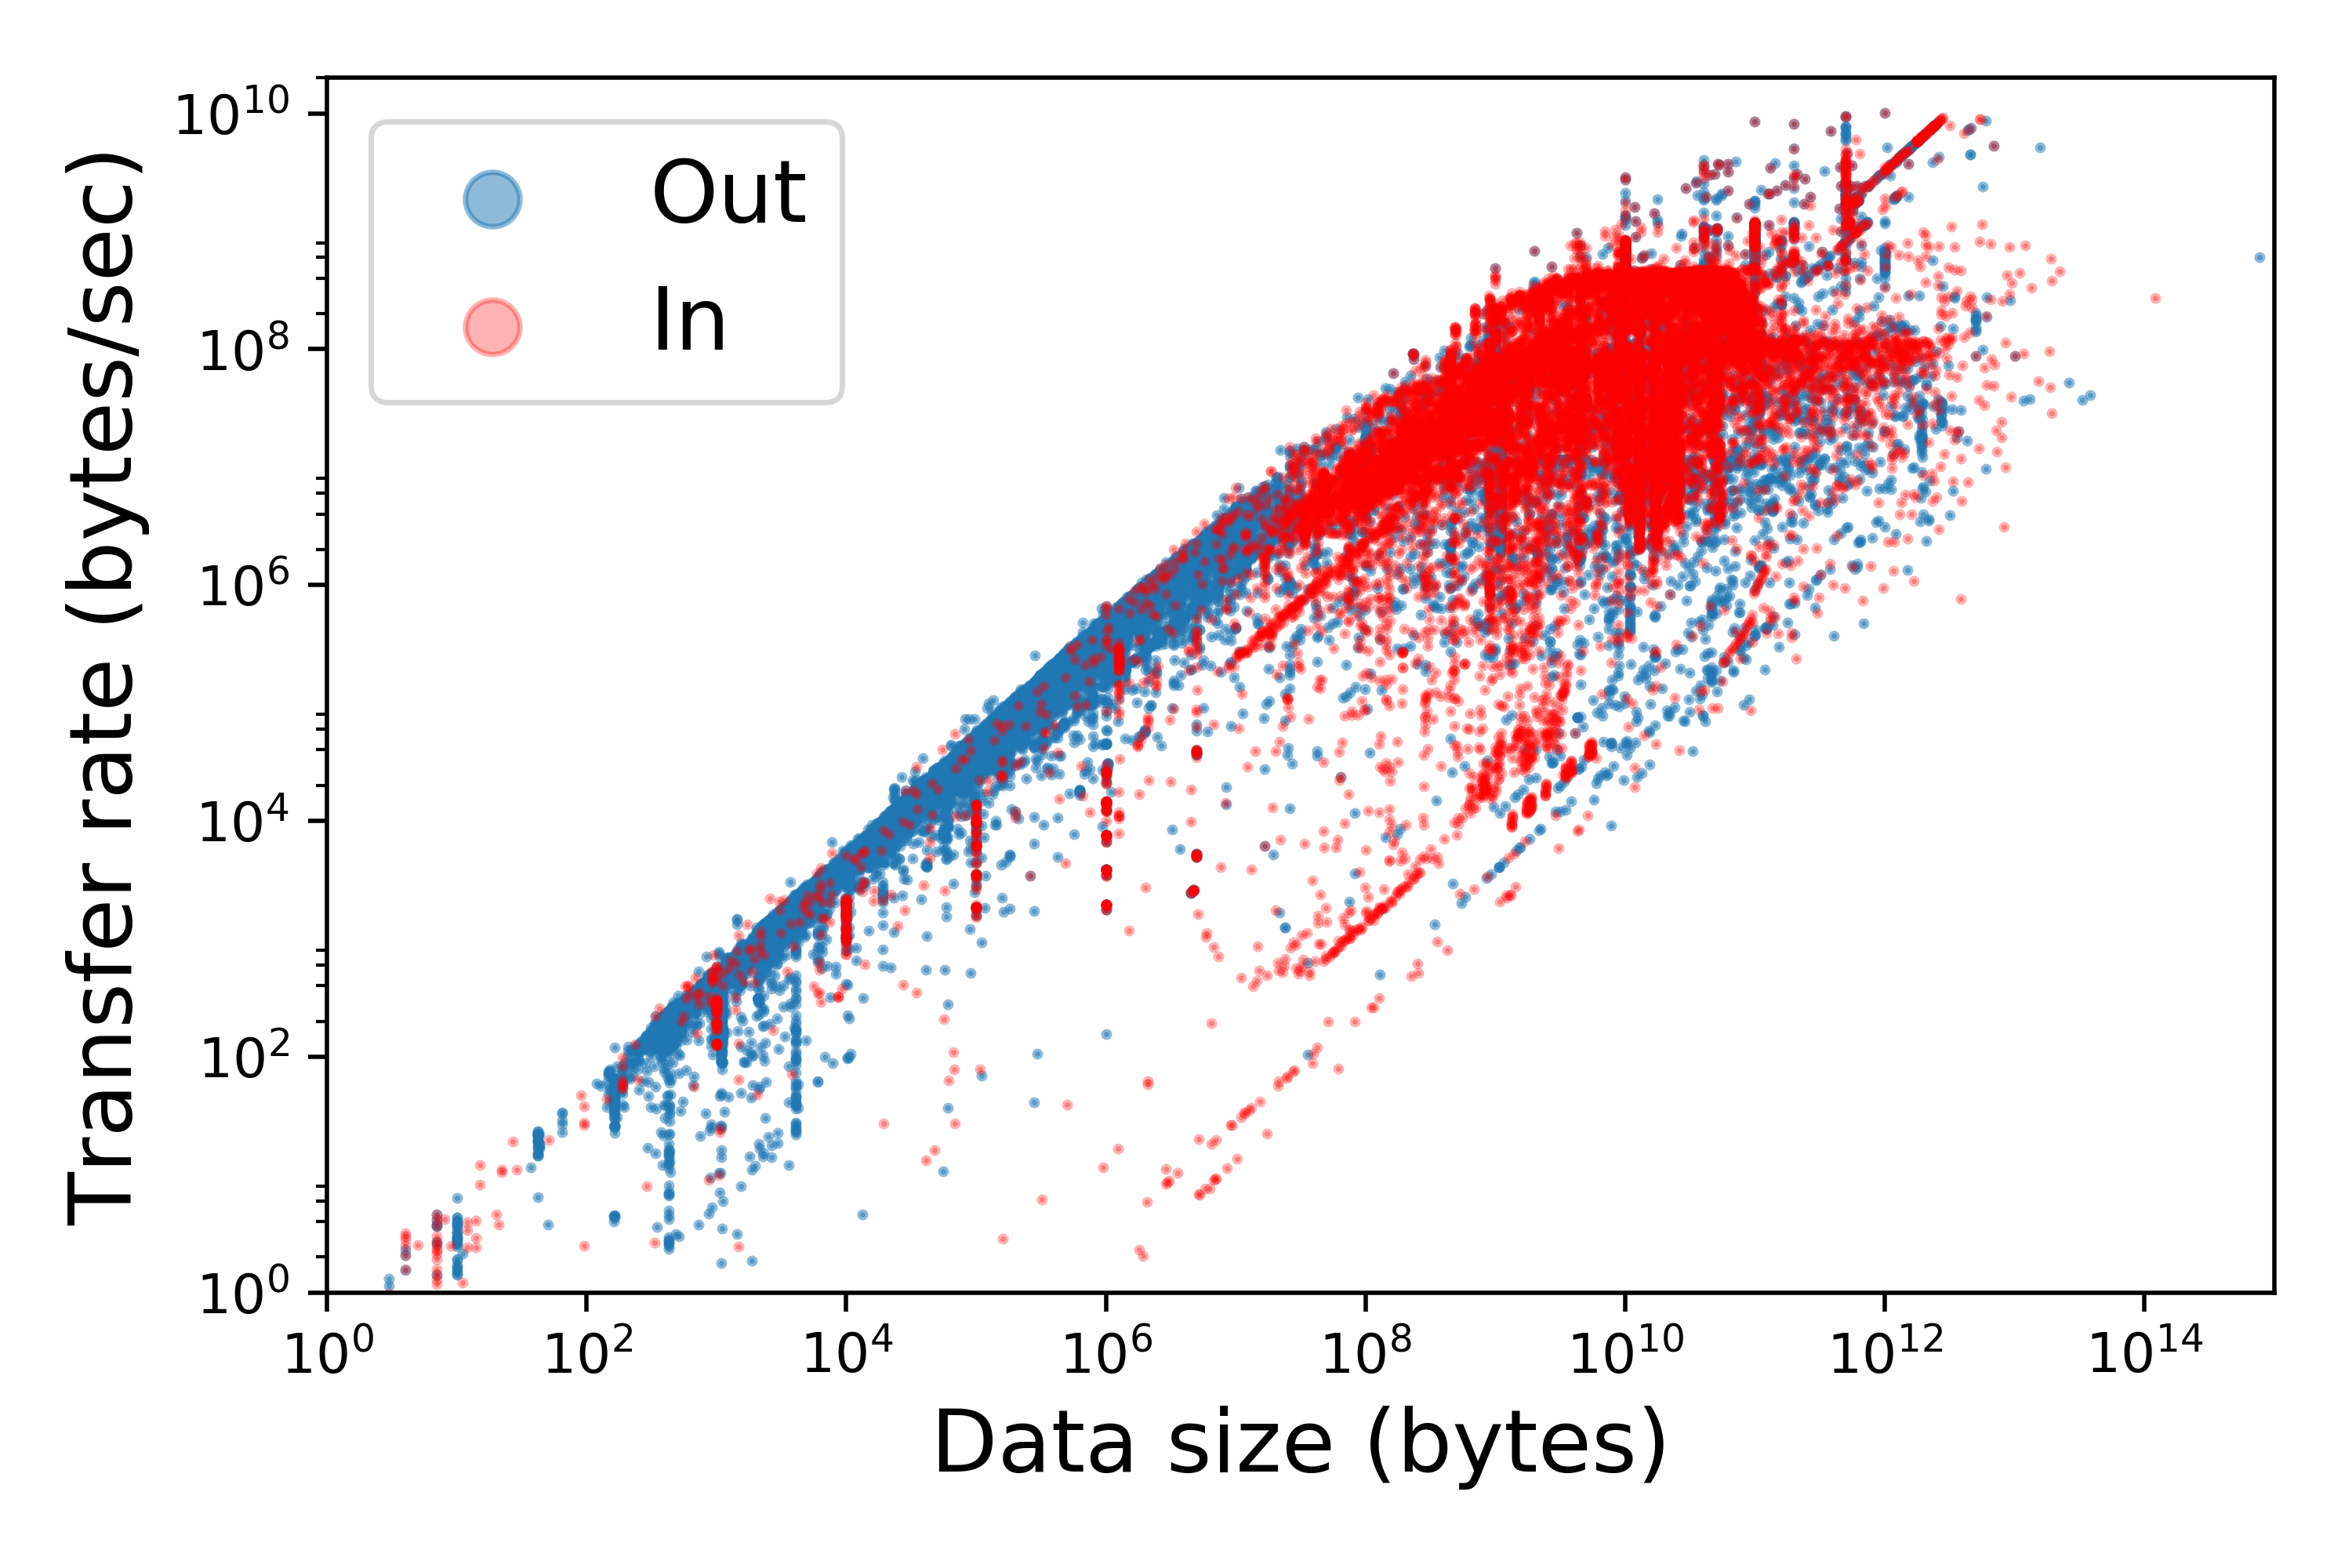
\includegraphics[width=0.47\textwidth,trim=0.14in 0.15in 0.15in 0.2in,clip]{Figures/petrel-size-time.png}
\vspace{-2ex}

\caption{Transfer rate vs.\ data size.
Each point represents a single transfer request, which may involve many files.
Incoming and outgoing transfers are distinguished.\label{fig:ratesize}}
\end{figure}

\begin{figure}
\centering
 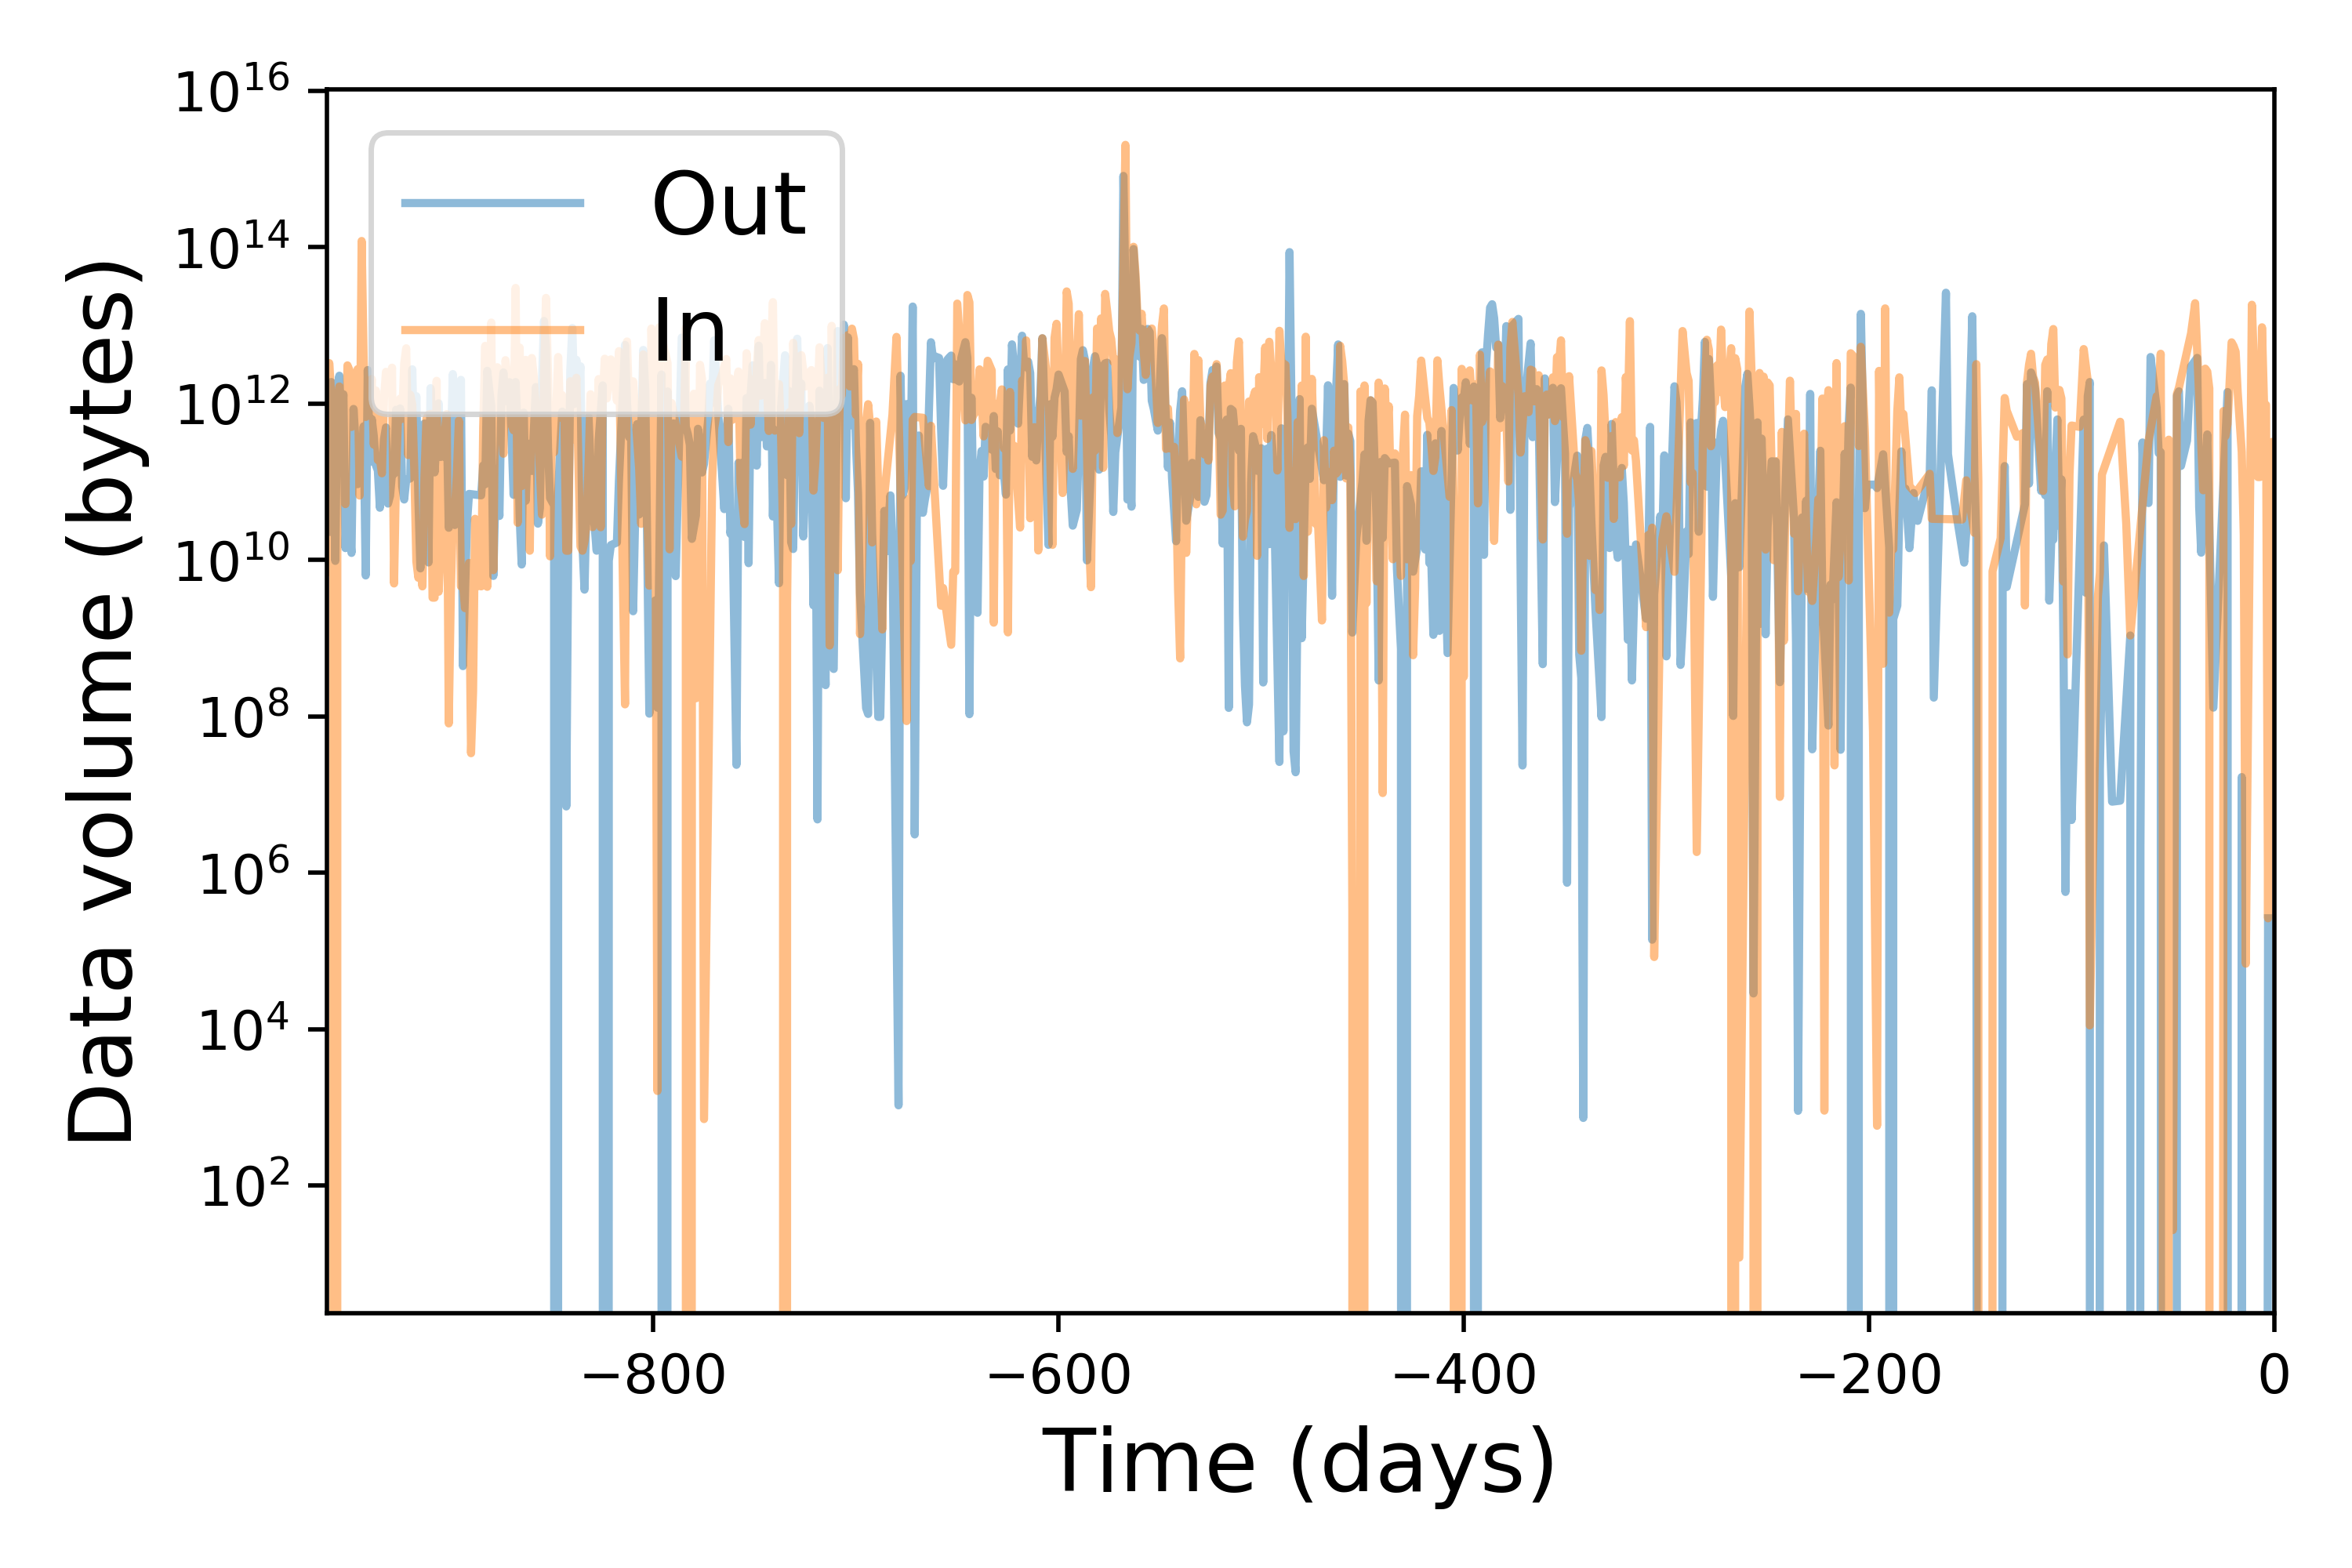
\includegraphics[width=0.47\textwidth,trim=0.14in 0.15in 0.15in 0.2in,clip]{Figures/petrel-bytes-day.png}
 
 \vspace{-2ex}

\caption{Input/output transfer volumes per day. The numbers on the x axis represent days prior to March 9, 2017.}
\label{fig:perday}
\end{figure} 


\begin{figure}
\centering
%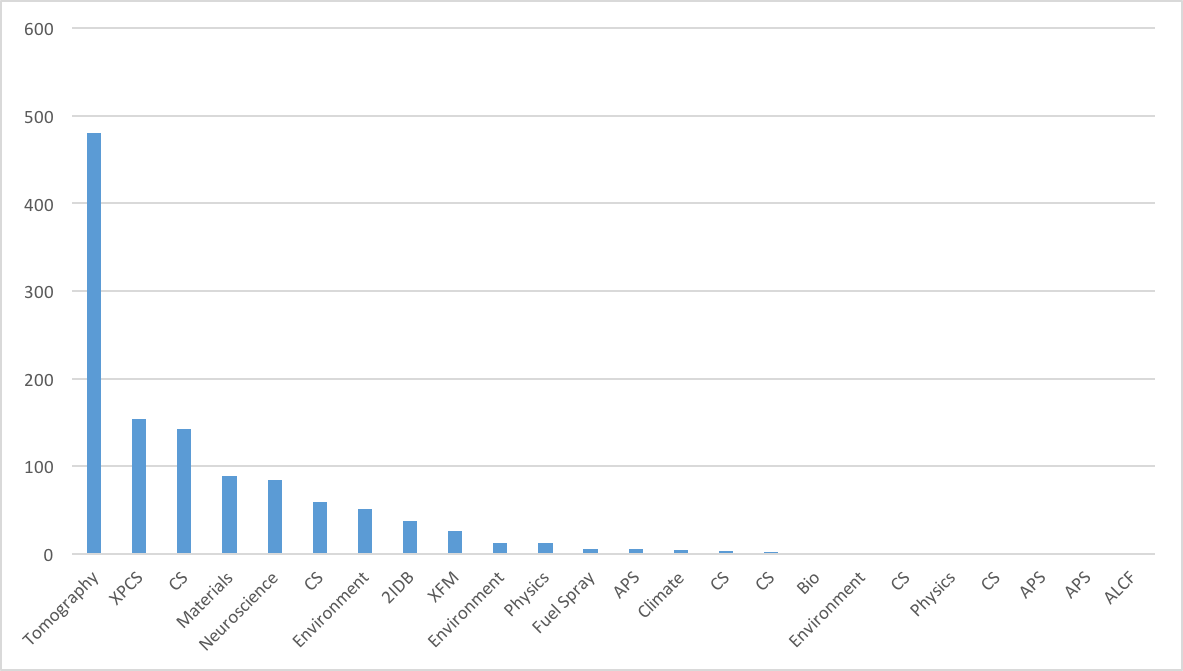
\includegraphics[trim=0.1in 0.1in 0.1in 0.1in,clip,width=\columnwidth]{Figures/usage.png}
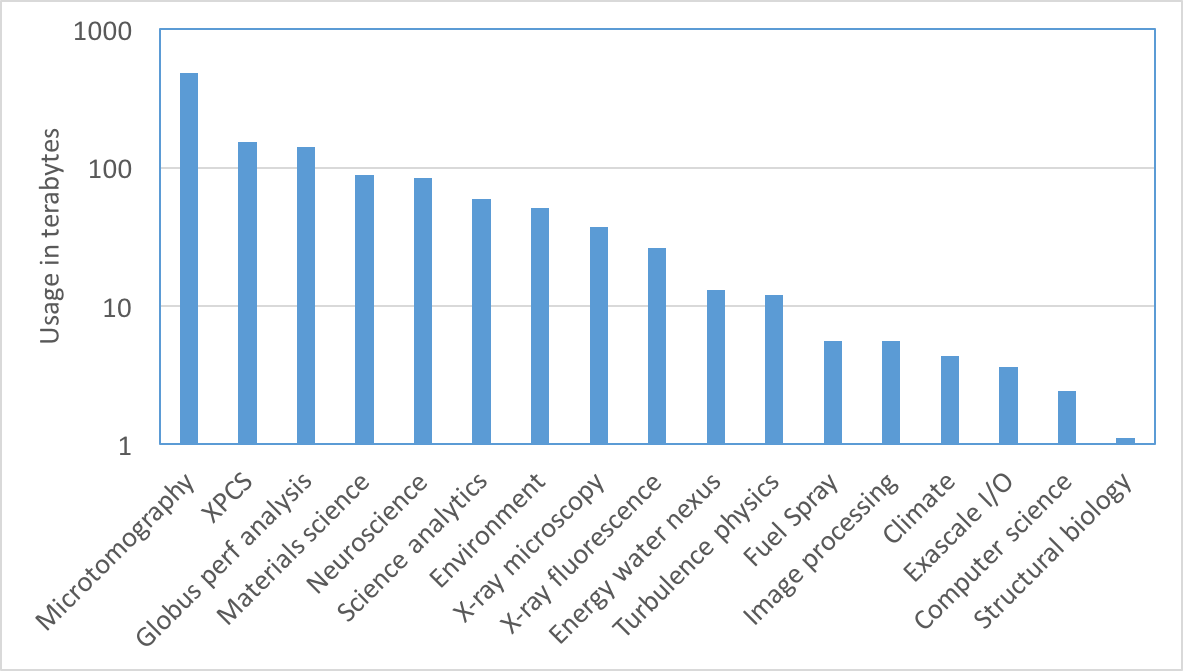
\includegraphics[trim=0.2in 0.1in 0.1in 0.1in,clip,width=\columnwidth]{Figures/PetrelUsage.png}

\vspace{-2ex}

\caption{Petrel storage consumption for projects using more than one terabyte, as of August 2017.
Note log scale. XPCS=X-ray photon correlation spectroscopy~\cite{shpyrko2014x}.\label{fig:usage3}}
\end{figure}

%\ian{Need to add reference to, and discussion of, Figures~\ref{fig:ratesize} and~\ref{fig:perday}.}


\section{Related Work}

Many systems have been developed to enable access to scientific data,
from GenBank~\cite{benson2012genbank} and the
Earth System Grid~\cite{doi:10.1175/2008BAMS2459.1} to Dataverse~\citep{meyer15pub}
and the Structural Biology Grid~\cite{meyer15pub}.
However, few follow the MRDP design pattern~\cite{BMRDP} in which data are located within a Science DMZ
for high-speed access.
Nor do the various portals~\citep{russell2001astrophysics}, 
science gateways~\citep{wilkins2008teragrid,lawrence2015science}, 
hubs~\citep{klimeck2008nanohub,mclennan2010hubzero}, 
and cloud-hosted systems~\cite{babuju16kotta} that have been developed to
enable on-demand access to science software.
But these systems could all be adapted to make use of Petrel-like capabilities.

A growing number of research computing centers and associated facilities operate
Science DMZs with associated DTNs for remote access to large storage~\cite{dart2014science}.
However, the storage itself is often accessible only by users with facility
accounts and is optimized for access by high-performance computing 
systems, with efficient DTN access a secondary consideration.
Petrel, in contrast, is optimized for high-speed network access and enables access by anyone.

Another approach to providing data services for science is to deploy a distributed file
system across collaborating systems and sites.
The Andrew File System~\cite{howard1988scale} has been used for this purpose.
Indiana University's Data Capacitor uses the Lustre parallel distributed file system~\cite{simms2007empowering}, a technology that was also explored on the TeraGrid~\cite{simms2007wide}.
MeDiCI leverages file system mechanisms to enable data caching on a metropolitan scale~\cite{Abramson2017}.
File system features such as caching can be useful,
but require tighter integration across participating systems, for example at the level of accounts.

Public and private cloud computing systems can also be used for online analysis of large datasets~\cite{heath2014bionimbus,CloudBook}.
Szalay advocates for specialized hardware platforms for online analysis of large simulation
datasets~\cite{szalay2014simulations}. 
Such approaches are largely orthogonal to the software architecture used here.

Petrel and the MRDP design pattern emphasize the placement of storage outside the HPC
center and programmatic control of data placement, 
access, and movement.
Logistical networking~\cite{beck2000logistical} takes this idea much further,
embedding storage throughout the network to be managed by specialized protocols~\cite{beck2002end}. 


\section{Conclusions}

We have described the realization of a high-speed data service within the Argonne 
Leadership Computing Facility (ALCF).
%designed for easy integration
%into application workflows. 
Our experience operating this service over the past three years suggests that this service
is indeed useful to many people.
As expected, researchers have used it to distribute data produced at Argonne in
computational and experimental 
studies and to stage data being brought to the Argonne Leadership Computing Facility (ALCF) for analysis.
Unexpected but pleasing is the variety of ways of which researchers have leveraged Petrel's API access to
integrate it into application
workflows.

Petrel's proximity to ALCF resources makes it easy for application workflows to transfer data to
high-performance computers for analysis.
However, some groups would like yet more tightly coupled computing to allow more efficient
responses to, for example, user requests for data subsets or analyses. 
We thus plan to enhance Petrel to support data analysis as well as access.
Care must be taken when so doing to address security concerns. 
Access to ALCF production resources requires an approval process and issuance of a
CRYPTOCard hardware access token.
Petrel, in contrast, is treated more like a web server, allowing access by anyone who can authenticate
with an approved credential.
One promising approach is to allow general access only for predefined analysis requests,
while requiring two-factor authentication for user-specified analyses.

\section*{Acknowledgments}

The Argonne Leadership Computing Facility is a DOE Office of Science User Facility supported under contract DE-AC02-06CH11357.
%We thank the Globus team for the development of the technologies described here.
%and participants in ``Building the Modern Research Data Portal'' workshops for their feedback.
This work was also supported in part by NSF grant ACI-1148484 and by the DOE under contract DE-AC02-06CH11357.

%\newpage

\bibliographystyle{ACM-Reference-Format}
\bibliography{petrel} 

\end{document}
